\section{Electronics}

\subsection{Grounding and shielding}

In a comprehensive noise analysis, different configurations for the grounding were studied to define and validate the final scheme. The signal from the aluminum readout strip is input to the FSSR2 ASIC. The returns of the floating high and low voltage supplies are isolated from the Hall B ground. To maintain the reference voltage level of the carbon fiber, the copper mesh on one side of the bus cable is connected at the hybrid area of the HFCB to the return line of the low voltage. Modules are read out by the FSSR2 ASICs located on the hybrid area of the HFCB. Power and readout connections are made at the L1C. There is no coupling of the power or return lines of different modules -- each module is independent of the other modules. All modules are electrically isolated from the detector support structure. Each crate in the system has a safety ground. To shield against electromagnetic interference, the cable shields -- signal, power, slow control, and pulser -- of each module are connected together at the L1C. The L1Cs of all modules are located at the entrance of the Faraday cage, and from each of the L1Cs a cable connects the shields to the Faraday cage, which in turn are connected by a single cable directly to the Hall B central ground (see Fig.~\ref{fig:shielding}). The SVT is placed inside a Faraday cage that comprises the cold plate, a forward disk, and a cylindrical carbon shell. 

Common mode noise is of particular concern in digital read-out systems as it cannot be measured on an event-by-event basis and thus a correction is impossible. It can only be estimated statistically. It is important to ensure that the input noise of the modules does not increase with services successively added to the system, as that would indicate problems in the grounding scheme and common-mode noise has been introduced into the system. The analysis of the common mode noise validated the decisions made on grounding and shielding of the HFCB and the detector.

\begin{figure}[hbt] 
\centering 
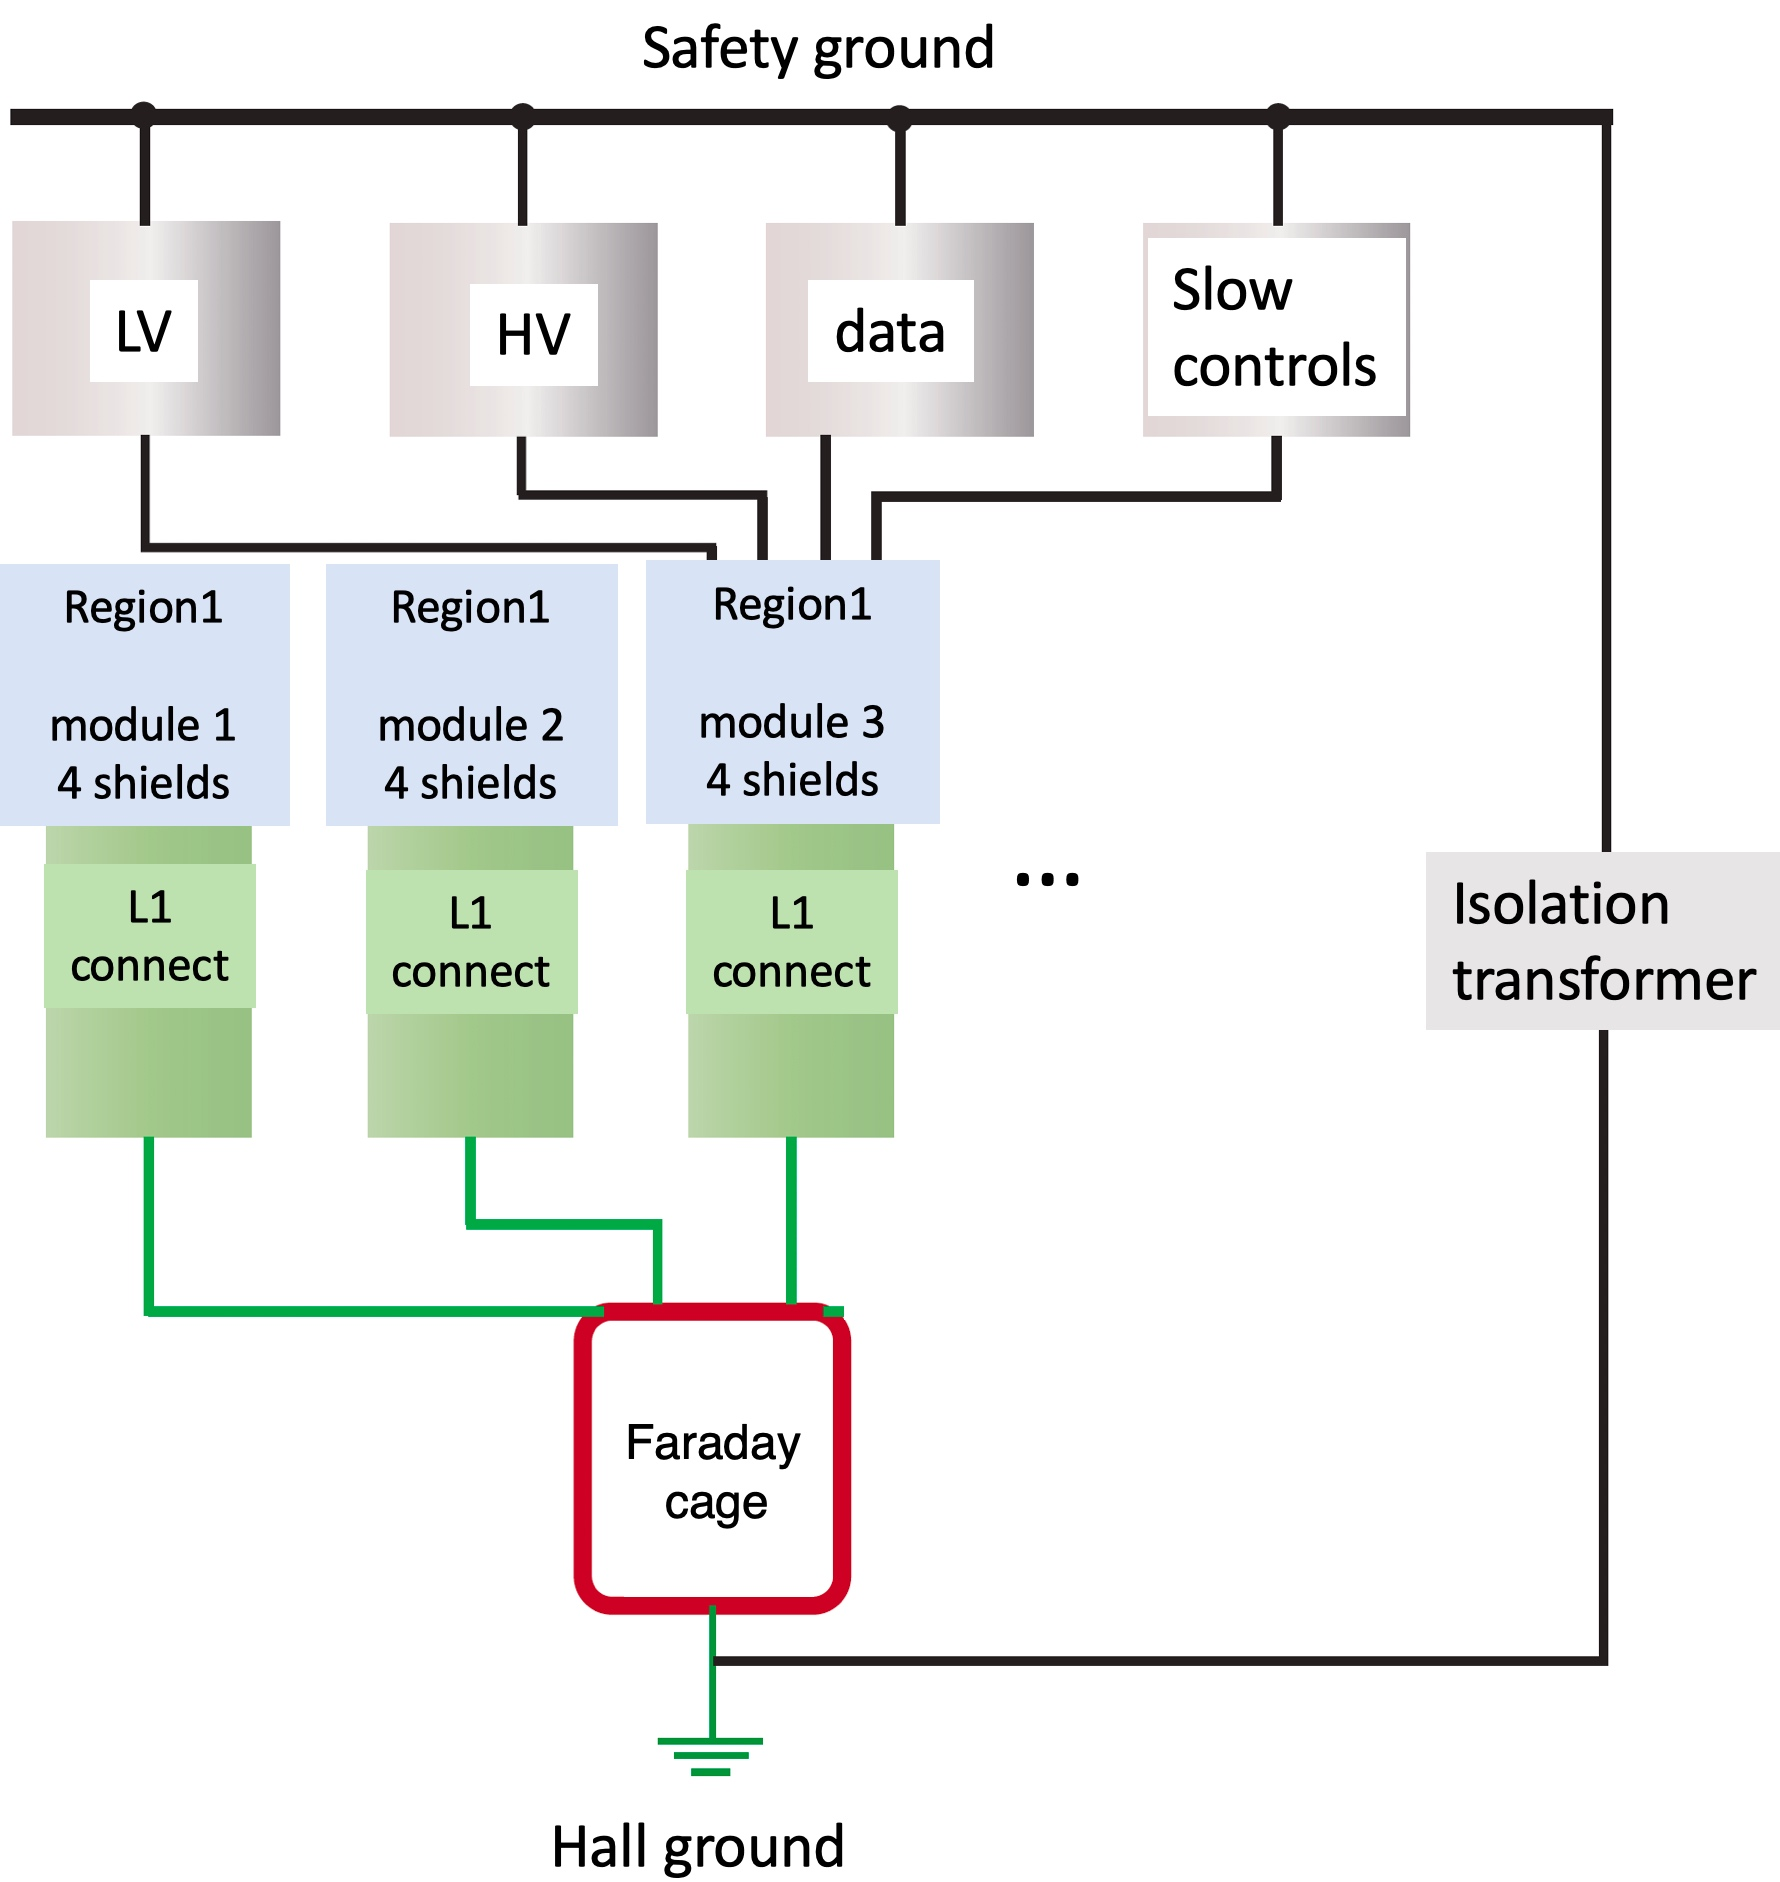
\includegraphics[width=1.0\columnwidth,keepaspectratio]{shielding.jpg}
\caption{SVT grounding scheme.}
\label{fig:shielding}
\end{figure}

\subsection{Power supplies}

Each side of a module has a high voltage channel, 80 V (40 $\mu$A), and two low voltage channels, 2.5 V (0.3 A). To power the FSSR2 ASICs and to bias the modules, Wiener's Universal Multi-channel Low and High Voltage System (MPOD) crates are used. The crates are 19 inches tall, rack-mountable, and capable of housing 10 low voltage Wiener cards or 10 high voltage ISEG cards, or a combination of the two (see Fig.~\ref{fig:mpod-crate}). The output voltage channels of the cards are floating. All power supply channels have programmable voltages, ramp rates, and limits. Hardware limits on voltage and current can be set on each card. Local control of the crate and cards is available on the LCD front panel; remote control is facilitated by a 10/100 Ethernet connection. 

\begin{figure}[hbt] 
\centering 
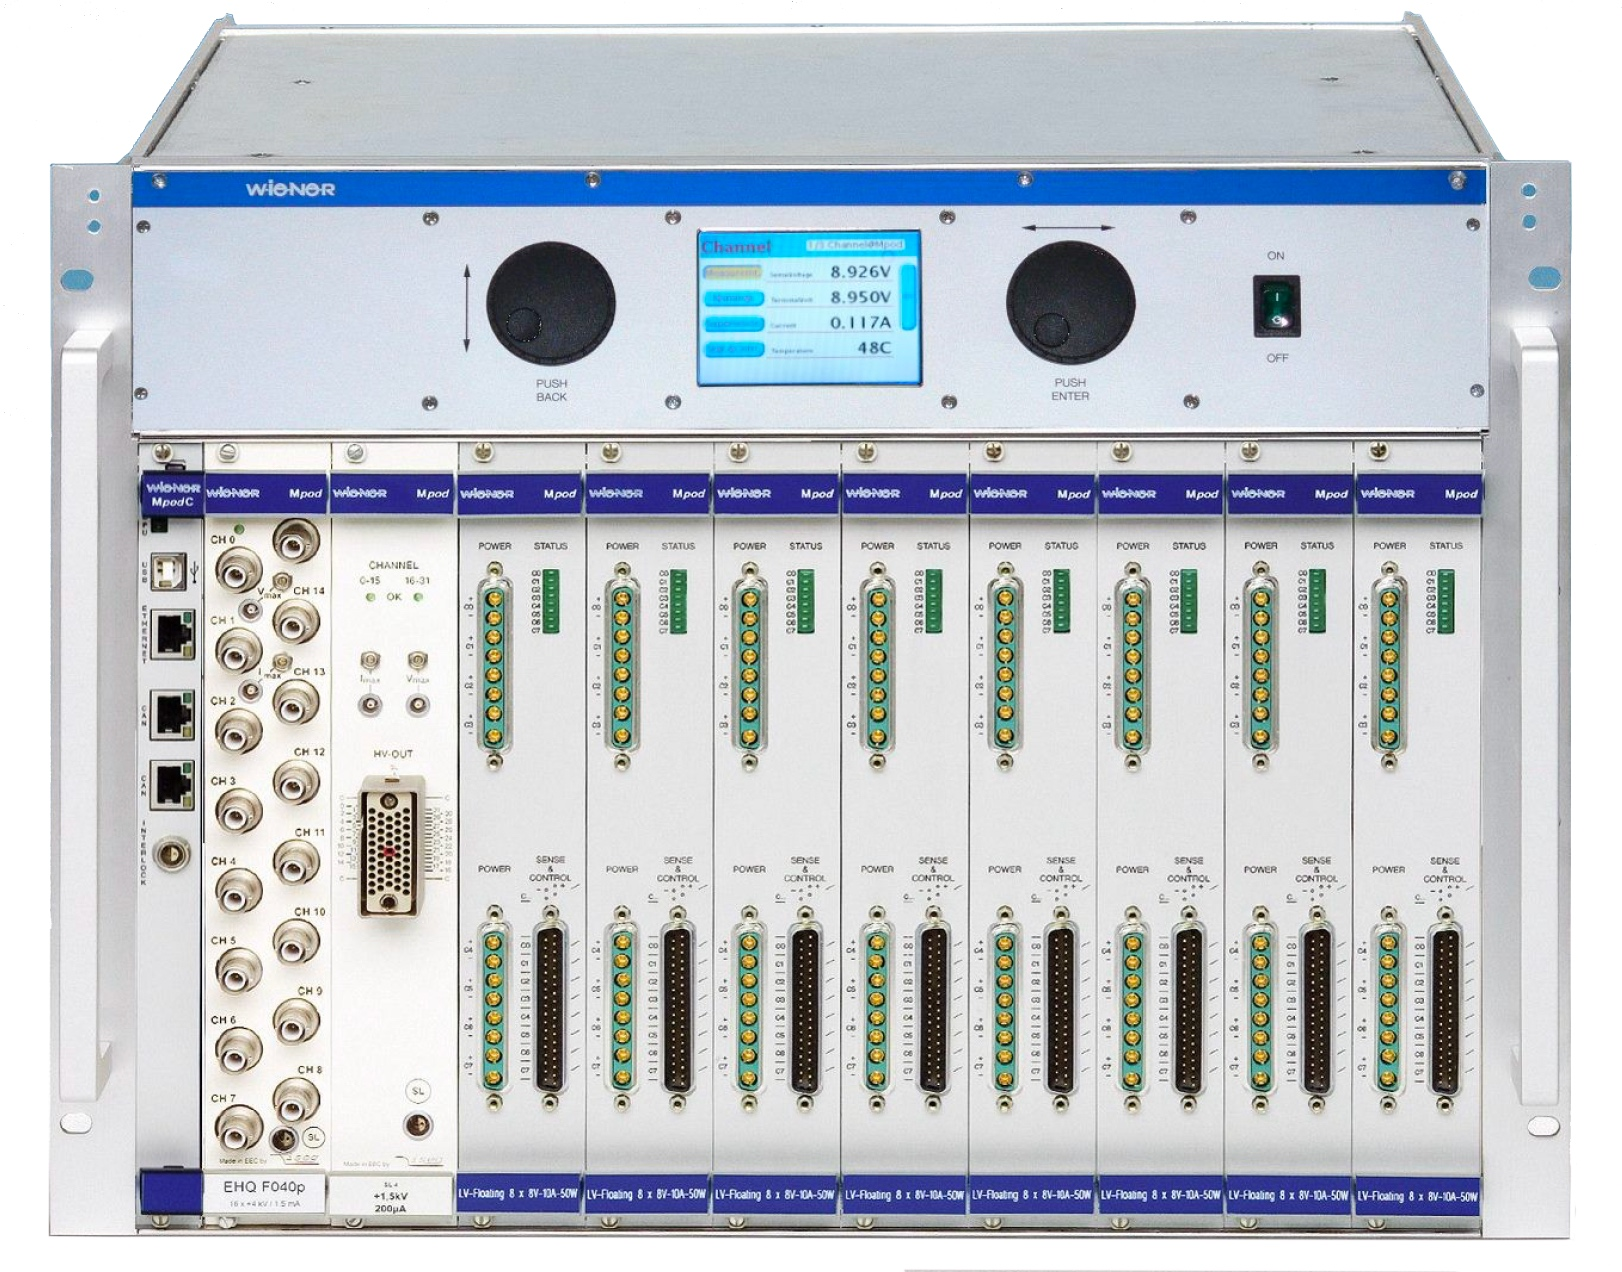
\includegraphics[width=1.0\columnwidth,keepaspectratio]{mpod-crate.jpg}
\caption{Wiener MPOD LX crate with mixed low and high voltage modules.}
\label{fig:mpod-crate}
\end{figure}

For low voltage, the Wiener eight-channel low voltage cards are used. These cards have a peak-to-peak voltage (Vpp) ripple of 10 mV and are capable of providing up to 8 V at 5 A per channel via a 2 x 37-pin, sub-D connector. Each output channel has a 12-bit voltage setting and measurement resolution, as well as a 12-bit current monitoring resolution. To bias the modules, the ISEG high precision, 16-channel high voltage cards are used. These cards have a Vpp ripple of 5 mV and are capable of providing up to 500 V at 10 mA via a Redel multi-pin connector. Each output channel has a 21-bit voltage setting and measurement resolution, as well as a 21-bit current monitoring resolution. Clean power, provided by shielded isolation transformers, is used for the high and low voltage power supplies.

